 \section{Nary DataType Relationship ODP}\begin{description}
\item [CLASSIFICATION:] Extension.

\item [MOTIVATION:] Numerical values can have different aspects. For example, a boiling point has a temperature value, a pressure, etc. This simple ODP should be used to model those cases.

\item [AIM:] To represent a datatype value with more than one aspect.

\item [STRUCTURE:] See Figure \ref{odp:Nary_DataType_Relationship_abstract}.
\begin{figure}[]\centering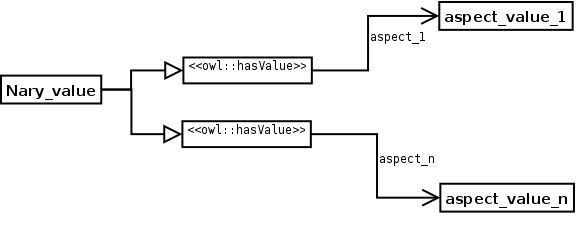
\includegraphics[width=\textwidth]{Catalogue/Nary_DataType_Relationship_abstract}\caption{\label{odp:Nary_DataType_Relationship_abstract} Abstract structure of the Nary DataType Relationship ODP.}\end{figure}

\item [SAMPLE:] See Figure \ref{odp:Nary_DataType_Relationship_instance}.
\begin{figure}[]\centering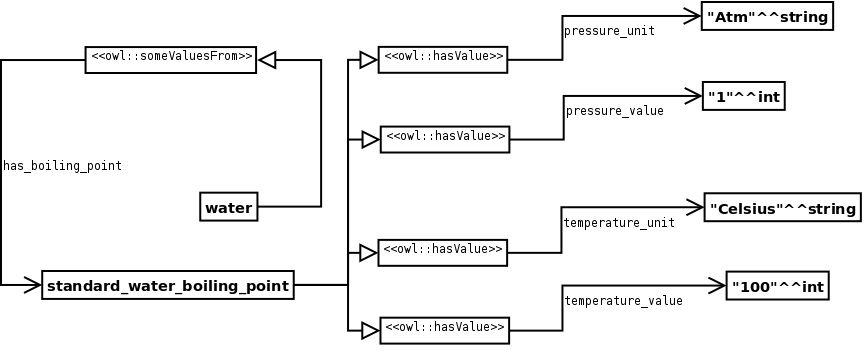
\includegraphics[width=\textwidth]{Catalogue/Nary_DataType_Relationship_instance}\caption{\label{odp:Nary_DataType_Relationship_instance} Sample structure of the Nary DataType Relationship ODP.}\end{figure}

\item [ELEMENTS:] The original value is reified (decomposed) in all the neccesary data type properties and values.

\item [IMPLEMENTATION:] The first step is to choose the datatype value that needs to be reified and create a class for it (e.g. StandardWaterBoilingPoint), then add a restriction (e.g. [Water HasBoilingPoint some StandardWaterBoilingPoint]) and all the neccesary datatype properties and restrictions to the reified class (e.g. [StandardWaterBoilingPoint partial HasUnit value celsius], [StandardWaterBoilingPoint partial  HasValue value 100], etc.).

\item [RESULT:] After the reification a value with different aspects is represented in the ontology.

\item [RELATED ODPS:] Nary Relationship.

\item [REFERENCES: ] ~\begin{itemize}
\item \url{http://www.cs.man.ac.uk/~stevensr/menupages/ontologies.php}
\item Bijan Parsia and Michael Smith. Quantities in OWL. OWLed 2008 EU.\end{itemize}
\item [URL: ] \url{http://www.gong.manchester.ac.uk/odp/owl/Extension_ODP/Nary_DataType_Relationship.owl} \end{description}